\begin{enumerate}\itemsep=-0.5em
    \item Temperatura (fuera y dentro del invernadero).
    \item Humedad relativa (fuera y dentro del invernadero).
    \item Luz o radiación solar (fuera y dentro del invernadero).
    \item Ventilación.
    \item Humedad de suelo.
    \item Temperatura de suelo.
    \item Fecha y hora de las mediciones de cada variables.  
    \item Zona geográfica. 
\end{enumerate}
\subsubsection{Temperatura (fuera y dentro del invernadero)}
La temperatura es una magnitud física que indica la energía interna de un
cuerpo, o de un sistema termodinámico en general. Esta propiedad termodinámica
únicamente describe un estado macroscópico.
La temperatura se define como la medida de la energía cinética media de las
moléculas que la forman. Es decir, los movimientos de las partículas en su
interior.
Por otro lado, se puede definir según la mecánica estadística, como la derivada
de la energía respecto a la entropía a volumen constante.

\subsubsection{Humedad relativa (fuera y dentro del invernadero)}

La humedad es una variable física definida formalmente como la cantidad de agua
disuelta en un gas o absorbida en un sólido.  Es una variable importante en
muchos ámbitos; por ejemplo, en procesos de fabricación que deben ser
ejecutados respetando condiciones de humedad especificas para garantizar los
productos. A veces la clave está en la humedad del aire ambiental, y otras en
la humedad de los productos mismos. 
\subsubsection{Luz o radiación solar (fuera y dentro del invernadero)}

La radiación solar se puede considerar el factor ambiental más importante en
los cultivos bajo invernadero, pues influye en procesos relacionados con la
fotosíntesis, los balances de agua y energía, y el crecimiento y desarrollo del
cultivo. Por tal motivo, el manejo de la radiación solar en la producción bajo
invernadero es sin duda una de las actividades más importantes en la
Horticultura Protegida, dicha importancia se sustenta en la relación directa
que existe entre la producción de materia seca y rendimiento con la cantidad de
radiación interceptada por el cultivo. 

La radiación solar es la fuente de
energía utilizada por las plantas en el proceso de fotosíntesis, y la
eficiencia de su aprovechamiento por las plantas va a depender de la longitud
de onda que esta presenta.


En la actualidad existen varios tipos de cubiertas de plástico, mallas sombra y
pantallas, mediante las cuales es posible modificar la calidad y cantidad de
energía luminosa en los invernaderos, sin embargo, existen consideraciones para
lograr el mejor aprovechamiento de la radiación solar. 

\begin{enumerate}
    \item Los materiales usados como cubierta en los invernaderos, salvo
        excepciones, deben ser transparentes a las radiaciones luminosas para
        permitir el paso de la luz visible. 

    \item Todos los materiales empleados para cubiertas de invernaderos
        reflejan una fracción de la luz que reciben del sol, que va del 20 – 30
        \%, generalmente. Al diseñar un invernadero, debe evitarse la formación
        de zonas sombreadas de las mismas estructuras, al proyectar e incidir
        en el interior, siendo estas lo más delgadas posibles para evitar
        interrumpir el paso de la luz. 

    \item En la actualidad existen materiales para cubiertas que difunden la
        luz que pasa a través de ellos convirtiéndola en luz difusa, la cual
        tiene la particularidad de no emitir sombras y llegar a todas partes y
        en todas direcciones. 

    \item La cantidad de luz que penetra a los invernaderos depende de la
        orientación de los mismos y de la forma o diseño de la estructura, pero
        sobre todo del ángulo de la cubierta con respecto al sol. 

    \item Es recomendable que los materiales de cubierta de los invernaderos
        transmitan del 85 – 90 \% de la luz solar incidente.
\end{enumerate}

Extraído de
https://www.intagri.com/articulos/horticultura-protegida/importancia-de-la-radiacion-solar-en-la-produccion-bajo-invernadero
- Esta información es propiedad intelectual de INTAGRI S.C., Intagri se reserva
el derecho de su publicación y reproducción total o parcial.

\subsubsection{Ventilación}
El sistema de ventilación en un invernadero sustituirá el aire más caliente que
se encuentra en el interior por otra masa de aire más frío que procede del
exterior. De esta manera gran parte de la sobrecarga de calor puede evacuarse,
disminuyendo la temperatura y, a su vez, modificando la concentración de gases
y la humedad. Se puede adoptar dos sistemas de ventilación: ventilación
mecánica. y ventilación natural. El sistema de ventilación que se debe emplear
depende de las propiedades del edificio y del tipo de cultivo que se realice.

\begin{enumerate}
    \item Ventilación natural:

        En la ventilación natural, el aire caliente que se encuentra en el
        interior del invernadero asciende y sale al exterior por dos aperturas
        situada en la cubierta, mientras que la admisión se realiza desde dos
        aperturas en la parte baja de las fachadas laterales. De esta forma se
        crea un flujo de aire que abarca todo el recinto interior. Para este
        tipo de ventilación son necesarias grandes aberturas, entre un 15 \% y
        un 25 \% de la superficie de la cubierta, y no permite controlar la
        incidencia de la velocidad del aire sobre las plantas.
    \item Ventilación mecánica simple:

        La ventilación mecánica se basa en la renovación del aire instalando
        ventiladores electromecánicos en la cubierta o más parte alta de una
        fachada lateral del invernadero, mientras que las entradas de aire que
       proviene del exterior se localizan en la parte baja de la pared
        opuesta.  Con este sistema la temperatura mínima interior no suele
        exceder de la del aire exterior.  

\end{enumerate}
\subsubsection{Humedad de suelo}
Unos niveles suficientes de humedad del suelo son una condición importante para
la formación adecuada de las plantas y el alto rendimiento de los cultivos.
Para la planta, el agua no sólo sirve como agente de restauración de la
humedad, sino también como regulador de la temperatura. En el proceso de
termorregulación, la planta evapora hasta el 99\% del agua obtenida, utilizando
sólo entre el 0,2\% y el 0,5\% para la formación de la masa vegetativa. Por lo
tanto, es fácil comprender que la planta tiene diferentes necesidades de
humedad según las condiciones climáticas y las etapas de crecimiento.
\subsubsection{Temperatura de suelo}
La temperatura es una propiedad que posee un efecto muy importante sobre los
organismos y sobre los procesos de alteración química de la fracción mineral
del suelo. Cada especie cultivada posee un rango propio de aptitud para la
germinación de la semilla, por ejemplo.  

La mayor parte de la energía calorífica que recibe el suelo procede de la
energía solar. En un clima templado, y por término medio, se estima que el
suelo recibe 144 calorías $día^{-1}* cm^{-2}$.  Obviamente, este valor varía con la
latitud, la época del año, la nubosidad, la orientación de la ladera y la
cubierta vegetal. 

La temperatura del suelo depende del balance de energía térmica absorbida,
emitida y reflejada \ref{fig:temperaturasuelo} Por lo tanto, la capacidad del suelo para
elevar su temperatura dependerá de una serie de variables intrínsecas (color,
humedad, calor específico, drenaje, renovación de la atmósfera del suelo, etc.)
y extrínsecas (humedad atmosférica, nubosidad, partículas en suspensión en la
atmósfera, precipitación, viento, relieve, vegetación, etc.). De manera más
detallada, los principales factores que influyen sobre la absorción de energía
solar por el suelo, son los siguientes: 

\begin{enumerate}
    \item El ángulo de incidencia de los rayos solares. La temperatura
        alcanzada es mayor cuando los rayos inciden de manera perpendicular al
        suelo. Este factor varía con la latitud (la temperatura alcanzada es
        mayor en el ecuador y disminuye cuando nos acercamos a los polos;
        ), la estación (los rayos solares en nuestras latitudes
        llegan con mayor inclinación en invierno que en verano) y
        el momento del día (la máxima perpendicularidad se alcanza al mediodía)
        . También como consecuencia de la orientación del sol, en
        nuestra latitud, las laderas orientadas al sur reciben más insolación
        que las orientadas al norte.  
    \item Las nubes atenúan la intensidad de
        la radiación solar. Sin embargo, pueden emitir radiación infrarroja, lo
        que es perceptible durante la noche.  La nubosidad minimiza la
        oscilación térmica entre el día y la noche.  
    \item Los suelos de color
        oscuro absorben mayor cantidad de energía térmica que los de color
        claro.  
    \item La humedad del suelo puede regular la temperatura, ya que
        el agua es un conductor del calor más rápido que la tierra, pero posee
        una gran inercia térmica. Por esta razón, los suelos más húmedos se
        calientan y enfrían más lentamente que un suelo seco. Por otra parte,
        la evaporación contribuye al mantenimiento de una temperatura más
        fresca.   
    \item La conductividad térmica del aire es muy
        baja. Por esta razón, los horizontes superficiales, si están bien
        aireados, difunden mal el calor hacia los horizontes inferiores, de
        modo que el suelo se calienta y enfría más rápidamente que un suelo
        poco poroso.  
    \item La vegetación y los restos de hojarasca (la capa de
        residuos vegetales del suelo se denomina frecuentemente como mulch)
        proporcionan una sombra que reduce el calentamiento del suelo durante
        el día. Además, pueden actuar como un aislante que evita la pérdida de
        energía térmica durante la noche.  En nuestras latitudes, la superficie
        de los suelos desprovistos de vegetación puede alcanzar los 40ºC en
        verano, con lo que se detiene la actividad biológica y se frenan los
        procesos edafogénicos.  
\end{enumerate}
\begin{figure}[H]
    \centering
    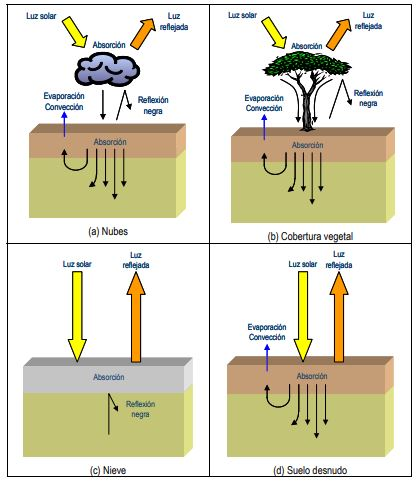
\includegraphics[width=\textwidth, keepaspectratio,
    heigh=7cm]{images/temperaturasuelo.JPG}
    \caption{Comportamiento de la temperatura en funciones de los distintos
    parámetros listados. }
    \label{fig:temperaturasuelo}
\end{figure}

\subsubsection{Localización}

Para determinar la zona donde estará ubicado el invernadero se
consideran los siguientes parámetros.

\begin{enumerate}
    \item Sanidad del terreno.

        Verificar que el terreno esté en excelentes condiciones e indagar sobre
        su historial. En el caso de siembras de tomate, evitar en lo posible
        sembrar en terreno donde anteriormente se hayan cultivado especies como
        pimiento o berenjena entre otros, los cuales pertenecen a la familia
        botánica del tomate (solanáceas), cuyas plagas y enfermedades
        generalmente son las mismas. Así mismo, evitar terrenos que
        anteriormente hayan sido usados como basureros o en otras actividades
        que puedan haber causado contaminación al suelo
    \item Fertilidad del terreno. 

        Se debe realizar un análisis del suelo para evaluar sus condiciones
        físicas y su composición química y microbiológica, que permita
        determinar si reúne las condiciones adecuadas para el desarrollo del
        cultivo.
    \item Drenaje del terreno. 

        Se debe seleccionar el mejor suelo con un buen drenaje y fertilidad. Un
        alto nivel freático puede limitar considerablemente la producción de
        tomate, principalmente por el ataque de enfermedades.
    \item Disponibilidad y calidad de agua de riego. 

        El invernadero debe estar cerca a fuentes de agua de excelente calidad,
        libre de contaminantes químicos y microbiológicos; debe existir un
        tanque de reserva para emergencias o épocas de sequía. El productor
        debe prever la cantidad de agua que será necesaria durante el
        desarrollo del cultivo, así como tener en cuenta los medios para su
        conducción y distribución.
    \item Historial de la información climática de la zona.

        En lo posible tener información acerca del comportamiento climático de
        la región: temperaturas máximas y mínimas tanto diurnas como nocturnas,
        comportamiento de la humedad relativa en la madrugada y en las horas de
        la tarde, velocidad y dirección del viento, horas y cantidad de los
        niveles de radiación, cantidad anual y máximo de mm/hora de las
        lluvias, y presencia de heladas, granizo y fenómenos naturales.

    \item Adecuada ventilación. 
    
        Se debe ubicar el invernadero en zonas donde exista suficiente
        ventilación para favorecer la remoción del aire húmedo o caliente desde
        su interior y de esta manera evitar la alta o baja humedad relativa que
        favorece el desarrollo de enfermedades, plagas, desórdenes fisiológicos
        y problemas de calidad y productividad en la planta. Cuando predominan
        vientos demasiado fuertes, también se producen condiciones
        desfavorables para el desarrollo de las plantas, especialmente
        condiciones de humedad relativa baja, por lo tanto será necesaria la
        ubicación de barreras vivas para disminuir la velocidad del viento.
    \item Luminosidad. 

        Se debe evitar ubicarlo cerca de árboles altos, construcciones o
        barreras geográficas como montañas que impidan la entrada de luz al
        invernadero.
    \item Pendiente del terreno. 

        Lo ideal es ubicar el invernadero en zonas de topografía plana
        adecuando el drenaje del terreno, pero si el terreno presenta alguna
        pendiente ésta no debe superar el 20%.
    \item Orientación. 

        Es importante ubicar el invernadero en sentido norte sur o de acuerdo a
        los ángulos de radiación para lograr la máxima penetración de la luz y
        minimizar el sombrío de las plantas a lo largo del día.
    \item Calidad de la estructura. 

        Lo ideal es construir un invernadero con materiales duraderos, como el
        acero galvanizado; en caso de utilizar madera o guadua se recomienda
        que éstas sean sometidas a algún tratamiento de inmunización para
        incrementar su vida útil.

\end{enumerate}

